\documentclass[aspectratio=169]{beamer}
\usetheme{Madrid}
\usecolortheme{default}
\usepackage[utf8]{inputenc}
\usepackage[T5]{fontenc}
\usepackage{graphicx}
\usepackage{hyperref}
\usepackage{booktabs}

\setbeamertemplate{caption}[numbered]
\renewcommand{\figurename}{Hình}
\renewcommand{\thefigure}{2.\arabic{figure}}

\title[Buổi 2: AI, Blockchain \& Big Data]{Trí tuệ Nhân tạo cho Kế toán \\ \vspace{0.3cm} \Large Buổi 2: AI, Blockchain và Dữ liệu lớn trong Kinh tế - Tài chính}
\author{Đại học Đông Á}
\date{\today}

\begin{document}

% SLIDE 1: TRANG BÌA
\begin{frame}
    \titlepage
\end{frame}

% SLIDE 2: NỘI DUNG CHƯƠNG TRÌNH
\begin{frame}{Nội dung Chương trình Buổi học (135 Phút)}
    \tableofcontents
\end{frame}

% SLIDE 3: MỤC TIÊU BÀI HỌC (LO)
\begin{frame}{Mục tiêu Bài học (Lesson Objectives - LO)}
    \begin{itemize}
        \item \textbf{LO 2.1 - Hiểu bản chất Tiền mã hóa:} Nắm vững khái niệm Bitcoin, tiền mã hóa, hệ thống thanh toán điện tử ngang hàng.
        \item \textbf{LO 2.2 - Công nghệ Blockchain:} Hiểu sổ cái công khai phân tán, hợp đồng thông minh, và ứng dụng blockchain trong tài chính.
        \item \textbf{LO 2.3 - Metaverse \& DeFi:} Khám phá vũ trụ ảo (metaverse) và tài chính phi tập trung (DeFi), ứng dụng NFT.
        \item \textbf{LO 2.4 - Dữ liệu lớn (Big Data):} Nắm vững đặc trưng 4 chữ V của Big Data, và phân biệt giữa khoa học dữ liệu, AI, ML, DL.
        \item \textbf{LO 2.5 - Quy trình Khai phá Dữ liệu:} Nắm vững vòng đời khoa học dữ liệu từ thu thập, làm sạch, mô hình hóa đến đánh giá mô hình.
    \end{itemize}
\end{frame}

% ==============================================================================
% SECTION 1: Tiền mã hóa, Bitcoin & Ứng dụng Blockchain trong Tài chính
% ==============================================================================
\section{1. Tiền mã hóa, Bitcoin \& Ứng dụng Blockchain trong Tài chính}

% SLIDE 4
\begin{frame}{1.1 Bitcoin: Hệ thống thanh toán điện tử mật mã}
    \begin{itemize}
        \item \textbf{Sự ra đời:} Được giới thiệu bởi Satoshi Nakamoto vào thời điểm diễn ra cuộc khủng hoảng tài chính toàn cầu (2008-2009).
        \item \textbf{Đặc điểm cốt lõi:} Là một loại tiền tệ phi tập trung (decentralized), được bảo vệ bằng mật mã (cryptography).
        \item \textbf{Thuận lợi:} Dễ dàng trao đổi ngang hàng (peer-to-peer exchange) mà không cần qua trung gian.
        \item \textbf{Bản chất:} Hoạt động dựa trên nền tảng khách (client-based) qua phần mềm mã nguồn mở.
    \end{itemize}
\end{frame}

% SLIDE 5
\begin{frame}{1.2 Đặc tính Phi tập trung \& Ngang hàng}
    \begin{itemize}
        \item \textbf{Sự khác biệt với Tiền pháp định (Fiat Money):} Không phụ thuộc vào tổ chức phát hành tập trung (như Ngân hàng Nhà nước).
        \item \textbf{Tạo giá trị:} Giá trị được tạo ra bởi niềm tin và sự chấp nhận của cộng đồng người dùng mạng lưới.
        \item \textbf{Kinh tế học mạng lưới (Network economics):} Các sản phẩm được tạo ra và giá trị được gia tăng thông qua quy mô hoạt động trên toàn cầu thay vì sự kiểm soát của một doanh nghiệp duy nhất.
    \end{itemize}
\end{frame}

% SLIDE 6
\begin{frame}{1.3 Bitcoin dưới góc nhìn Pháp lý \& Tòa án}
    \begin{itemize}
        \item \textbf{Tòa án Tối cao Tây Ban Nha (2019):} Từ chối công nhận Bitcoin là tiền tệ hợp pháp (legal tender) mà coi nó là một "tài sản vô hình" (incorporeal asset).
        \item \textbf{Tòa án Công lý Châu Âu (CJEU):} Phán quyết Hedqvist coi Bitcoin là một loại tiền ảo và các bên có thể chấp nhận nó như một phương tiện thanh toán phi doanh nghiệp.
        \item \textbf{UKJT (Anh Quốc):} Coi tiền mã hóa là "tài sản" (property) có khả năng xác định, sở hữu, chuyển nhượng và có giá trị.
    \end{itemize}
\end{frame}

% SLIDE 7
\begin{frame}{1.4 Lập luận của Tổng Biện lý về Tiền tệ}
    \begin{itemize}
        \item \textbf{3 Chức năng cốt lõi của Tiền tệ:}
        \begin{enumerate}
            \item Phương tiện trao đổi (Medium of exchange).
            \item Công cụ lưu trữ giá trị (Store of value).
            \item Đơn vị kế toán (Unit of account).
        \end{enumerate}
        \item \textbf{Góc nhìn về Bitcoin:} Tổng Biện lý cho rằng Bitcoin không phải là tiền điện tử (e-money) vì nó "chậm chạp, tốn kém và không thể dùng thanh toán hóa đơn thường nhật", không được quản lý bởi thực thể trung tâm.
    \end{itemize}
\end{frame}

% SLIDE 8
\begin{frame}{1.5 Nghịch lý của Tiền mã hóa}
    \begin{itemize}
        \item \textbf{Tầm nhìn ban đầu:} Giải phóng hoạt động tài chính khỏi nhà nước và loại bỏ chi phí đại diện (agency costs) của các tổ chức trung gian.
        \item \textbf{Nghịch lý thực tế:} Để phát triển mạnh mẽ và ổn định, Bitcoin lại cần các trung gian tài chính (sàn giao dịch, ETFs) nhằm cung cấp thanh khoản và khám phá giá.
        \item \textbf{Hệ quả:} Điều này tạo ra chính những vấn đề đại diện (agency problems) mà Bitcoin ban đầu được thiết kế để tránh khỏi.
    \end{itemize}
\end{frame}

% SLIDE 9
\begin{frame}{1.6 Tiền kỹ thuật số của Ngân hàng Trung ương (CBDC)}
    \begin{itemize}
        \item \textbf{Phản ứng của Nhà nước:} Mặc dù tiền mã hóa cố gắng loại bỏ vai trò của chính phủ, các quốc gia hiện đang bước chân vào không gian kỹ thuật số với \textbf{CBDC} (Central Bank Digital Currency).
        \item \textbf{Mục tiêu của CBDC:}
        \begin{itemize}
            \item Duy trì quyền kiểm soát cung tiền (monetary policy).
            \item Gia tăng bao trùm tài chính (financial inclusion).
            \item Đảm bảo mức độ tin cậy được hậu thuẫn bởi cơ quan quyền lực nhà nước (ví dụ: e-CNY, Digital Euro).
        \end{itemize}
    \end{itemize}
\end{frame}

% SLIDE 10
\begin{frame}{1.7 Sổ cái Công khai Phân tán (Distributed Ledger)}
    \begin{itemize}
        \item \textbf{Blockchain (Chuỗi khối):} Là một cơ sở dữ liệu phi tập trung khổng lồ chứa các định danh đặc trưng cho mỗi người dùng và mỗi Bitcoin.
        \item \textbf{Vai trò Công chứng viên (Public Notary):} Blockchain hoạt động như một hệ thống xác nhận giao dịch để lại dấu vết không thể xóa bỏ trong không gian mạng.
        \item \textbf{Lợi ích:}
        \begin{itemize}
            \item Chi phí giao dịch thấp hơn mạng lưới tài chính truyền thống (Swift).
            \item Ứng dụng rõ ràng nhất là hệ thống thanh toán và chuyển tiền xuyên biên giới.
        \end{itemize}
    \end{itemize}
\end{frame}

% SLIDE 11
\begin{frame}{1.8 Rủi ro: Sự Biến động \& Tính Pháp lý}
    \begin{itemize}
        \item \textbf{Tính Biến động (Volatility):} Giá trị tiền mã hóa biến động rất lớn, khiến chúng trở thành các khoản đầu tư nguy hiểm và thiếu tính ổn định làm công cụ lưu trữ giá trị.
        \item \textbf{Thiếu Cơ sở Pháp lý:} Là rào cản khổng lồ đối với sự đổi mới có trách nhiệm.
        \item \textbf{Rủi ro Hệ thống:} Nếu một loại tiền ảo được áp dụng rộng rãi nhưng không thể kiểm soát, nó có thể đe dọa đến sự ổn định của hệ thống tài chính vĩ mô.
    \end{itemize}
\end{frame}

% SLIDE 12
\begin{frame}{1.9 Cuộc đua Tiền ảo (Altcoins)}
    \begin{itemize}
        \item \textbf{Litecoin:} Tốc độ tạo khối nhanh hơn, sử dụng thuật toán "scrypt", giải mã qua CPU tiêu dùng.
        \item \textbf{Ethereum (2015):} Nền tảng phân tán hỗ trợ Hợp đồng Thông minh (Smart Contracts) và Ứng dụng Phân tán (DApps).
        \item \textbf{Zcash (2016) / Monero:} Tiền mã hóa bảo mật cao với cơ chế giao dịch ẩn danh (shielded transactions).
        \item \textbf{Ripple (XRP):} Mạng thanh toán toàn cầu tập trung vào đối tượng ngân hàng.
    \end{itemize}
\end{frame}

% SLIDE 13
\begin{frame}{1.10 Tính Minh bạch \& Có thể Kiểm toán của Blockchain}
    \begin{itemize}
        \item \textbf{Đặc tính Bất biến (Immutability):} Dữ liệu một khi được ghi lại trên chuỗi khối sẽ không thể bị thay đổi hay giả mạo.
        \item \textbf{Lợi thế đối với Kiểm toán viên:} 
        \begin{itemize}
            \item Mọi thành viên đều có thể truy cập một phiên bản thống nhất của sự thật (singular version of the truth).
            \item Góp phần chống lại các mối đe dọa mạng, đảm bảo tính toàn vẹn và mức độ an mật chưa từng có của số liệu.
        \end{itemize}
    \end{itemize}
\end{frame}

% SLIDE 14
\begin{frame}{1.11 Chuỗi khối \& AI: Cặp bài trùng của Tài chính}
    \begin{itemize}
        \item \textbf{Sự hội tụ quyền lực:}
        \begin{itemize}
            \item \textbf{Blockchain:} Cung cấp hạ tầng an toàn, minh bạch, dữ liệu sạch và đáng tin cậy.
            \item \textbf{AI:} Cung cấp năng lực phân tích dự đoán (predictive analytics) và ra quyết định tự động theo thời gian thực.
        \end{itemize}
        \item \textbf{Ứng dụng thực tế:}
        \begin{itemize}
            \item Hệ thống chống rửa tiền (AML), nhận biết khách hàng (KYC).
            \item Mô hình phát hiện gian lận bằng Đồ thị (GNN - Graph Neural Networks).
        \end{itemize}
    \end{itemize}
\end{frame}

% SLIDE 15
\begin{frame}{1.12 Hợp đồng Thông minh (Smart Contracts)}
    \begin{itemize}
        \item \textbf{Khái niệm:} Hợp đồng thông minh là các đoạn mã (code) tự động hóa và thực thi thỏa thuận khi các điều kiện định trước được thỏa mãn.
        \item \textbf{Vai trò:}
        \begin{itemize}
            \item Loại bỏ nhu cầu sử dụng các bên trung gian (luật sư, ngân hàng, công chứng).
            \item Đẩy nhanh tốc độ xử lý giao dịch và giảm thiểu rủi ro tranh chấp tài chính.
        \end{itemize}
        \item \textbf{Cố vấn Rô-bốt (Robo-advisors):} AI tự động đưa ra đề xuất đầu tư được cá nhân hóa dựa trên phân tích dữ liệu lịch sử khách hàng (giao kết trên Smart Contracts).
    \end{itemize}
\end{frame}


% ==============================================================================
% SECTION 2: Tài chính Phi tập trung (DeFi), NFT & Vũ trụ Ảo (Metaverse)
% ==============================================================================
\section{2. Tài chính Phi tập trung (DeFi), NFT \& Vũ trụ Ảo (Metaverse)}

% SLIDE 16
\begin{frame}{2.1 Giao dịch Thuật toán (Algorithmic Trading)}
    \begin{itemize}
        \item \textbf{AI trong Giao dịch Tài chính:} Thuật toán AI đang thay đổi động lực thị trường chứng khoán/tiền ảo bằng cách tự động hóa hoàn toàn quá trình phân tích và đặt lệnh.
        \item \textbf{Lợi ích:}
        \begin{itemize}
            \item Tốc độ khớp lệnh mili-giây (High-frequency trading).
            \item Giao dịch không bị chi phối bởi tâm lý sợ hãi (FOMO) hay tham lam của con người.
            \item Cải thiện tính thanh khoản và hiệu quả của các thị trường tài chính toàn cầu.
        \end{itemize}
    \end{itemize}
\end{frame}

% SLIDE 17
\begin{frame}{2.2 Vũ trụ Ảo (Metaverse) trong Tài chính}
    \begin{itemize}
        \item \textbf{Khái niệm:} Metaverse là một không gian ảo (ảo hóa bằng VR/AR và Blockchain) nơi con người có thể làm việc, giải trí và giao dịch tài chính như thế giới thực.
        \item \textbf{Crypto-Metaverse:} Vũ trụ ảo gắn liền với kinh tế học tiền mã hóa (crypto-economics), nơi tiền mã hóa là phương tiện thanh toán cốt lõi.
        \item Môi trường chính yếu cho việc hình thành, giao dịch và sở hữu các tài sản kỹ thuật số (Digital Assets).
    \end{itemize}
\end{frame}

% SLIDE 18
\begin{frame}{2.3 Bất động sản Ảo, Nghệ thuật Số \& Mã thông báo}
    \begin{itemize}
        \item Trong Metaverse, các sản phẩm sau đây được mua bán nhộn nhịp:
        \begin{itemize}
            \item \textbf{Nghệ thuật kỹ thuật số (Digital art):} Các bức tranh, nhạc phẩm độc bản.
            \item \textbf{Bất động sản ảo (Virtual real estate):} Mảnh đất ảo trong Decentraland, The Sandbox.
            \item \textbf{Mã thông báo trò chơi (Gaming tokens):} Tiền tệ trong GameFi (Play-to-Earn).
        \end{itemize}
        \item \textbf{Pháp lý:} Tại Ý, token được coi là "tài sản kỹ thuật số" (Bộ luật dân sự); tại Pháp, được coi là "tài sản vô hình".
    \end{itemize}
\end{frame}

% SLIDE 19
\begin{frame}{2.4 Tài chính Phi tập trung (DeFi) trong Metaverse}
    \begin{itemize}
        \item \textbf{DeFi (Decentralized Finance):} Cung cấp các dịch vụ tài chính truyền thống (cho vay, đi vay, gửi tiết kiệm lấy lãi, hoán đổi token) ngay trong không gian vũ trụ ảo mà không cần ngân hàng.
        \item \textbf{Lợi ích:}
        \begin{itemize}
            \item Tự động hóa qua Hợp đồng thông minh.
            \item Nâng cao sự bao trùm tài chính (financial inclusion).
            \item Loại bỏ các rào cản địa lý và chi phí giao dịch trung gian.
        \end{itemize}
    \end{itemize}
\end{frame}

% SLIDE 20
\begin{frame}{2.5 Fintech \& Ngân hàng Ảo (Virtual Banking)}
    \begin{itemize}
        \item \textbf{Virtual Banking:} Ngân hàng hoạt động trực tuyến 100\% mà không phụ thuộc vào bất kỳ chi nhánh/phòng giao dịch vật lý nào.
        \item \textbf{Đóng góp của Fintech \& Ngân hàng ảo:}
        \begin{itemize}
            \item Mở tài khoản và xác thực danh tính điện tử (eKYC) nhanh chóng.
            \item Phê duyệt khoản vay bằng thuật toán AI phân tích dữ liệu tự động thay vì nhân viên tín dụng.
            \item Thúc đẩy sự cạnh tranh, tạo thêm nhiều sản phẩm tài chính sáng tạo.
        \end{itemize}
    \end{itemize}
\end{frame}

% SLIDE 21
\begin{frame}{2.6 Tính tương tác \& Bề mặt Tấn công mạng}
    \begin{itemize}
        \item \textbf{Tính Tương tác (Interoperability):} Đặc tính chính của vũ trụ ảo cho phép người dùng mang tài sản ảo (ví dụ: trang phục NFT, tiền) từ nền tảng này sang nền tảng khác.
        \item \textbf{Rủi ro Bề mặt Tấn công (Attack Surface):}
        \begin{itemize}
            \item Chuyển đổi số tạo ra nhiều "cổng vào" (entry points) cho tin tặc.
            \item Các vụ tấn công phần mềm độc hại (Malware) và rò rỉ dữ liệu (Data breaches) tăng mạnh.
            \item Tập đoàn trở thành mục tiêu béo bở khi dữ liệu tập trung (data centralization) cao.
        \end{itemize}
    \end{itemize}
\end{frame}

% SLIDE 22
\begin{frame}{2.7 AI \& Nghệ thuật NFT (Non-Fungible Token)}
    \begin{itemize}
        \item \textbf{Bản chất của NFT:} Là mã thông báo không thể thay thế, được dùng để chứng nhận quyền sở hữu độc bản của một tài sản số.
        \item \textbf{Sự hội nhập của AI:}
        \begin{itemize}
            \item Tạo ra nghệ thuật kỹ thuật số tự chủ (AI-generated artworks).
            \item Quản lý đề xuất bán NFT (Recommender Systems) thông qua phân tích sở thích thị trường.
            \item Xác nhận tính nguyên bản (Authenticity) và phát hiện vi phạm bản quyền.
        \end{itemize}
    \end{itemize}
\end{frame}

% SLIDE 23
\begin{frame}{2.8 Vấn đề Đạo đức \& Bản quyền AI}
    \begin{itemize}
        \item \textbf{Sáng tạo là gì?} Là sản xuất ra ý tưởng/sản phẩm độc đáo và có giá trị. AI hiện đang đóng vai trò khởi xướng sự đổi mới (innovation).
        \item \textbf{Khoảng trống Pháp lý:}
        \begin{itemize}
            \item Ai sở hữu Quyền sở hữu trí tuệ (IPRs) cho một tác phẩm do AI vẽ hoàn toàn? Người viết prompt (lời nhắc), thuật toán AI, hay người lập trình ra AI đó?
            \item Vấn đề này rất nhạy cảm khi các tác phẩm nghệ thuật do AI tạo ra được mã hóa thành các mã thông báo (tokenized) và bán với giá cao.
        \end{itemize}
    \end{itemize}
\end{frame}

% SLIDE 24
\begin{frame}{2.9 Giao thoa giữa DeFi và NFT (Mã hóa Tài sản thực)}
    \begin{itemize}
        \item \textbf{NFT làm Tài sản thế chấp (Collateral):} 
        \begin{itemize}
            \item Người dùng có thể cầm cố một bức tranh NFT để vay tiền mã hóa trên nền tảng DeFi (không cần bán đứt).
        \end{itemize}
        \item \textbf{Mã hóa Tài sản Thế giới thực (RWA - Real World Assets):}
        \begin{itemize}
            \item Chứng thư sở hữu nhà, hàng xa xỉ phẩm, đồng hồ Rolex được mã hóa thành NFT.
            \item Tăng tính thanh khoản cho thị trường và mở rộng sự tham gia đầu tư.
            \item \emph{Thách thức:} Rủi ro biến động giá trị của tài sản không thể thay thế và khó khăn trong thẩm định giá.
        \end{itemize}
    \end{itemize}
\end{frame}

% ==============================================================================
% SECTION 3: Khoa học Dữ liệu & Hệ sinh thái Dữ liệu Lớn (Big Data)
% ==============================================================================
\section{3. Khoa học Dữ liệu \& Hệ sinh thái Dữ liệu Lớn (Big Data)}

% SLIDE 25
\begin{frame}{3.1 Khoa học Dữ liệu (Data Science) - Sự Thổi phồng}
    \begin{itemize}
        \item \textbf{Bối cảnh thập kỷ qua:} Từ khóa "Data Science" đã trở thành hiện tượng toàn cầu, hứa hẹn giảm thiểu kém hiệu quả và kích thích tăng trưởng cực đại cho tổ chức.
        \item \textbf{Nghề nghiệp Hấp dẫn nhất Thế kỷ 21} (Theo Harvard Business Review, 2012).
        \item \textbf{Định nghĩa Khoa học Dữ liệu:}
        \begin{itemize}
            \item Là lĩnh vực liên ngành kết hợp Thống kê, Toán học, Khoa học Máy tính và Chuyên môn Nghiệp vụ (Domain Expertise) để trích xuất những hiểu biết sâu sắc (Insights) nhằm tạo ra giá trị kinh doanh.
        \end{itemize}
    \end{itemize}
\end{frame}

% SLIDE 26
\begin{frame}{3.2 Nhà Khoa học Dữ liệu (Data Scientist)}
    \begin{columns}
        \column{0.55\textwidth}
        \begin{itemize}
            \item \textbf{Toán \& Thống kê:} Giúp xây dựng và kiểm định mô hình.
            \item \textbf{Lập trình (Hacking/Computer Science):} Giúp xử lý dữ liệu tự động, triển khai mô hình.
            \item \textbf{Chuyên môn Nghiệp vụ (Domain Expertise):} Giúp hiểu ý nghĩa con số và kết quả bài toán tài chính.
            \item \textbf{Cân bằng:} Cần hội tụ đủ 3 yếu tố này; nếu thiếu Kỹ năng nghiệp vụ, việc phân tích sẽ bị lạc hướng (Danger Zone).
        \end{itemize}
        
        \column{0.45\textwidth}
        \begin{figure}
            \centering
            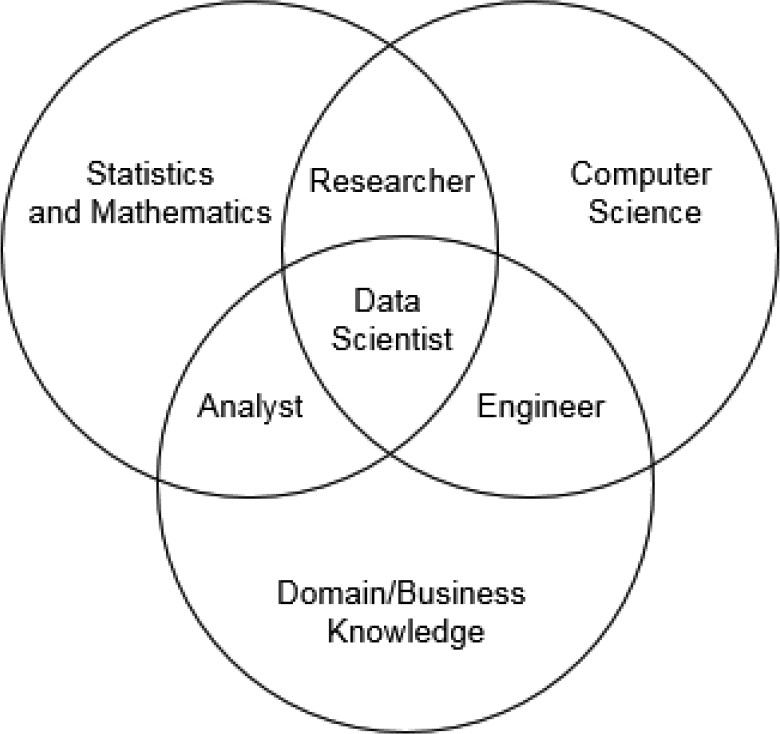
\includegraphics[width=\textwidth,height=0.75\textheight,keepaspectratio]{../../Figures/Buoi_02B/Figure 6.2 Data scientist Venn diagram.jpeg}
            \caption{Biểu đồ Venn các kỹ năng Data Science}
        \end{figure}
    \end{columns}
\end{frame}

% SLIDE 27
\begin{frame}{3.3 Phân tích Dữ liệu (Analytics) vs. Khoa học Dữ liệu}
    \begin{itemize}
        \item \textbf{Ranh giới Mờ nhạt nhưng khác biệt:}
        \item \textbf{Nhà Phân tích Dữ liệu / Phân tích Kinh doanh (Data/Business Analyst):}
        \begin{itemize}
            \item Tập trung sử dụng chuyên môn nghiệp vụ để trực quan hóa, phân tích quá khứ và báo cáo (Tạo ra Insights).
            \item Công cụ: Excel, SQL, PowerBI.
        \end{itemize}
        \item \textbf{Nhà Khoa học Dữ liệu (Data Scientist):}
        \begin{itemize}
            \item Vai trò rộng hơn, đòi hỏi kỹ năng lập trình (Python/R) và xây dựng mô hình Học máy (Machine Learning) để dự báo tương lai.
        \end{itemize}
    \end{itemize}
\end{frame}

% SLIDE 28
\begin{frame}{3.4 Mối quan hệ AI - ML - DL - Data Science}
    \begin{columns}
        \column{0.55\textwidth}
        \begin{itemize}
            \item \textbf{Trí tuệ Nhân tạo (AI):} Máy tính bắt chước hành vi thông minh (học hỏi, lập luận).
            \item \textbf{Học máy (ML):} Thuật toán thống kê giúp máy tự học quy luật từ dữ liệu.
            \item \textbf{Học sâu (DL):} Xử lý tự động trích xuất đặc trưng với dữ liệu phi cấu trúc.
            \item \textbf{Khoa học dữ liệu (Data Science):} KHÔNG nằm trong AI, mà nó \textbf{bao hàm} việc ứng dụng AI/ML/DL để giải quyết bài toán kinh doanh.
        \end{itemize}
        
        \column{0.45\textwidth}
        \begin{figure}
            \centering
            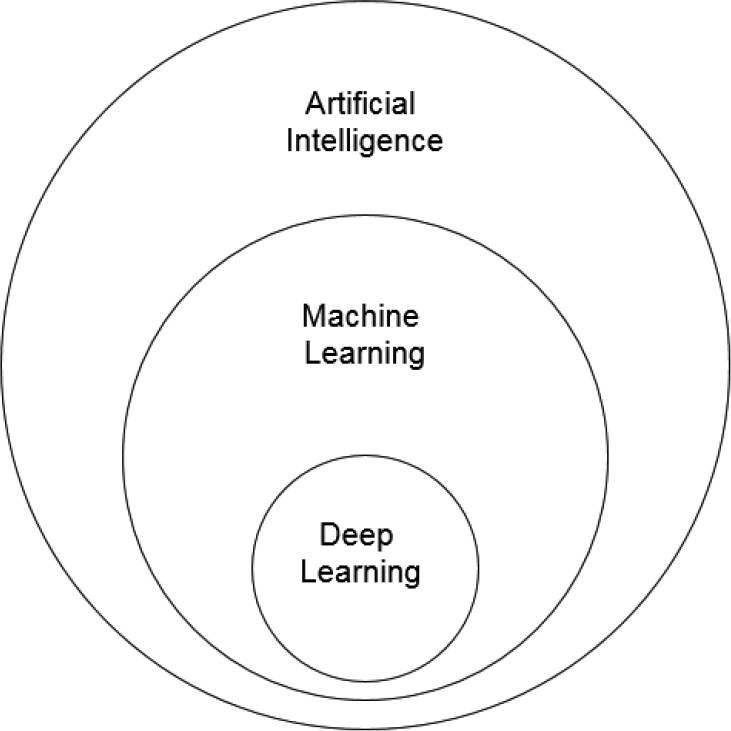
\includegraphics[width=\textwidth,height=0.75\textheight,keepaspectratio]{../../Figures/Buoi_02B/Figure 6.3 AI, machine learning, and deep learning Venn diagram.jpeg}
            \caption{Biểu đồ AI, ML, DL}
        \end{figure}
    \end{columns}
\end{frame}

% SLIDE 29
\begin{frame}{3.5 Những gì KHÔNG phải là Khoa học Dữ liệu?}
    \begin{itemize}
        \item \textbf{AI, Học máy, Học sâu:} Bản thân chúng không cấu thành 1 nhánh của Khoa học dữ liệu. Hãy coi ML là "Bộ công cụ" (toolkit) thống kê mà Khoa học dữ liệu sử dụng.
        \item \textbf{Dữ liệu lớn (Big Data):} Khoa học dữ liệu có thể làm việc với Excel 1,000 dòng hoặc Hadoop 1 tỷ dòng. Big Data chỉ là "Nguyên liệu", không phải là "Khoa học dữ liệu".
    \end{itemize}
\end{frame}

% SLIDE 30
\begin{frame}{3.6 Dữ liệu lớn (Big Data) là gì?}
    \begin{itemize}
        \item \textbf{Định nghĩa:} Khối lượng dữ liệu khổng lồ, phức tạp mà các phần mềm cơ sở dữ liệu truyền thống (như Excel hay SQL đơn giản) không thể quản lý và xử lý kịp.
        \item \textbf{Nguồn phát sinh Big Data hàng ngày (Khoảng 2,5 Quintillion bytes/ngày):}
        \begin{itemize}
            \item Hoạt động mạng xã hội (Facebook, Twitter).
            \item Lịch sử tìm kiếm (Google), phát trực tuyến video (Netflix, YouTube).
            \item Thanh toán (Quẹt thẻ tín dụng, Mobile Banking).
            \item Dữ liệu từ thiết bị di động \& Internet vạn vật (IoT).
        \end{itemize}
    \end{itemize}
\end{frame}

% SLIDE 31
\begin{frame}{3.7 Đặc trưng 4 Chữ V của Dữ liệu Lớn (IBM)}
    \begin{itemize}
        \item \textbf{1. Volume (Khối lượng):} Kích thước khổng lồ của dữ liệu.
        \item \textbf{2. Velocity (Vận tốc):} Tốc độ dữ liệu được tạo ra liên tục (Thời gian thực - Real-time).
        \item \textbf{3. Variety (Đa dạng):} Các loại dữ liệu từ có cấu trúc (bảng biểu) đến phi cấu trúc (văn bản, âm thanh, hình ảnh).
        \item \textbf{4. Veracity (Tính Xác thực/Độ Tin cậy):} Chất lượng dữ liệu có bị nhiễu, sai sót, hay mơ hồ đối với phân tích không.
    \end{itemize}
\end{frame}

% ==============================================================================
% SECTION 4: Quy trình Mô hình hóa & Đánh giá Mô hình Học máy
% ==============================================================================
\section{4. Quy trình Mô hình hóa \& Đánh giá Mô hình Học máy}

% SLIDE 32
\begin{frame}{4.1 Vòng đời Dự án Khoa học Dữ liệu}
    \begin{columns}
        \column{0.45\textwidth}
        \begin{itemize}
            \item \textbf{Định nghĩa Vấn đề}
            \item \textbf{Thu thập Dữ liệu} (Data Ingestion \& Storage)
            \item \textbf{Chuẩn bị Dữ liệu} (Làm sạch \& Khám phá EDA)
            \item \textbf{Mô hình hóa} (Train \& Test)
            \item \textbf{Đánh giá Mô hình}
            \item \textbf{Thử nghiệm (Experimentation)} và Triển khai
        \end{itemize}
        
        \column{0.55\textwidth}
        \begin{figure}
            \centering
            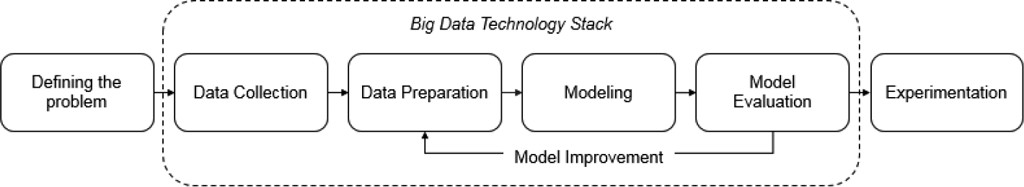
\includegraphics[width=\textwidth,height=0.8\textheight,keepaspectratio]{../../Figures/Buoi_02B/Figure 6.4 Data science project lifecycle.jpeg}
            \caption{Vòng đời Dự án Khoa học Dữ liệu}
        \end{figure}
    \end{columns}
\end{frame}

% SLIDE 33
\begin{frame}{4.2 Bước 1: Định nghĩa Vấn đề (Ví dụ: Nợ quá hạn)}
    \begin{itemize}
        \item Cần trả lời các câu hỏi nền tảng:
        \begin{itemize}
            \item Vấn đề kinh doanh là gì? (Giảm tỷ lệ nợ quá hạn vay tiêu dùng)
            \item Dữ liệu nào cần thiết? (Lịch sử thanh toán, số dư tài khoản, độ tuổi khách hàng)
            \item Định nghĩa sự thành công (KPI) ra sao? (Giảm 10\% nợ xấu)
        \end{itemize}
        \item Việc cấu trúc bài toán tốt ngay từ đầu quyết định toàn bộ sự thành công của dự án khoa học dữ liệu.
    \end{itemize}
\end{frame}

% SLIDE 34
\begin{frame}{4.3 Bước 2: Thu thập \& Phân loại Dữ liệu}
    \begin{columns}
        \column{0.4\textwidth}
        \begin{itemize}
            \item \textbf{Dữ liệu có cấu trúc:} Dạng bảng, SQL, hàng/cột rõ ràng.
            \item \textbf{Bán cấu trúc:} JSON, XML, file Log hệ thống.
            \item \textbf{Phi cấu trúc:} Hình ảnh (hóa đơn), âm thanh, video, văn bản tự do.
        \end{itemize}
        
        \column{0.6\textwidth}
        \begin{figure}
            \centering
            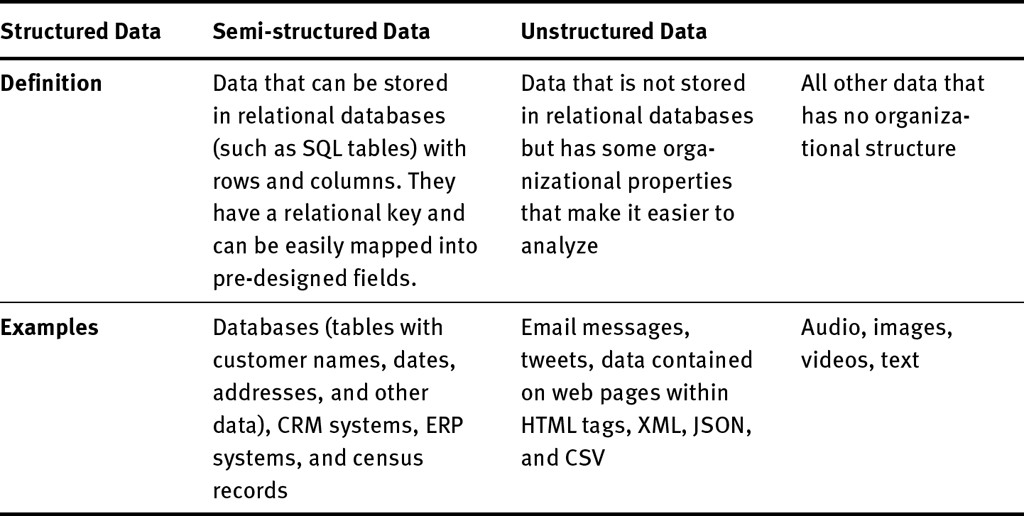
\includegraphics[width=\textwidth,height=0.7\textheight,keepaspectratio]{../../Figures/Buoi_02B/Table 6.1 Differences between Structured, Semi-Structured and Unstructured Data.jpeg}
            \caption{Phân loại Cấu trúc Dữ liệu}
        \end{figure}
    \end{columns}
\end{frame}

% SLIDE 35
\begin{frame}{4.4 Bước 3: Chuẩn bị Dữ liệu (Data Preparation)}
    \begin{itemize}
        \item \textbf{Dữ liệu thô (Raw data)} thường lộn xộn, thiếu sót và chứa lỗi (Giá trị NULL, trùng lặp).
        \item \textbf{Kiểm tra chất lượng dữ liệu (Data Quality Checks - QC):}
        \begin{enumerate}
            \item \textbf{Tính đầy đủ (Completeness):} Không bị thiếu cột, thiếu trường giá trị.
            \item \textbf{Tính chính xác (Accuracy):} Loại bỏ hoặc xử lý giá trị bất thường (Outliers).
            \item \textbf{Tính duy nhất (Uniqueness):} Khử trùng lặp (De-duplicate) theo Khóa chính (Ví dụ: ID khách hàng).
            \item \textbf{Tính nhất quán (Consistency):} Logic giữa các trường dữ liệu hợp lý.
            \item \textbf{Tính hợp lệ (Validity):} Chuẩn hóa định dạng (Ngày tháng, Text).
        \end{enumerate}
    \end{itemize}
\end{frame}

% SLIDE 36
\begin{frame}{4.5 Phân tích Dữ liệu Khám phá (EDA)}
    \begin{itemize}
        \item \textbf{Exploratory Data Analysis (EDA):} 
        \begin{itemize}
            \item Là bước tạo các thống kê mô tả (Mean, Median, Mode) và vẽ biểu đồ để tìm ra quy luật (patterns) tiềm ẩn của dữ liệu trước khi chạy thuật toán.
            \item Phân tích đơn biến (Univariate) và song biến (Bivariate).
        \end{itemize}
        \item \textbf{Nhận diện Biến Mục tiêu (Target Variable):}
        \begin{itemize}
            \item Biến kết quả kinh doanh mà ta muốn mô hình dự đoán. 
            \item Ví dụ bài toán phân loại nhị phân: Biến mục tiêu là trạng thái \texttt{Nợ quá hạn} (1) hoặc \texttt{Không nợ quá hạn} (0).
        \end{itemize}
    \end{itemize}
\end{frame}

% SLIDE 37
\begin{frame}{4.6 Phân loại Mô hình Học máy}
    \begin{itemize}
        \item \textbf{1. Học có giám sát (Supervised Learning):} Dữ liệu đã có "Nhãn mục tiêu" (Target).
        \begin{itemize}
            \item \textbf{Phân loại (Classification):} Dự báo danh mục rời rạc (Ví dụ: Nợ xấu / An toàn, Thư rác / Bình thường).
            \item \textbf{Hồi quy (Regression):} Dự báo số liên tục (Ví dụ: Dự báo Giá nhà, Doanh thu).
        \end{itemize}
        \item \textbf{2. Học không giám sát (Unsupervised Learning):} Tìm cấu trúc ngầm trên dữ liệu KHÔNG có mục tiêu (Không Nhãn).
        \begin{itemize}
            \item \textbf{Phân cụm (Clustering):} Gom nhóm đối tượng tương tự nhau (Phân khúc KH).
            \item \textbf{Luật liên kết (Association):} Tìm quy luật (Mua bia kèm tã lót).
        \end{itemize}
    \end{itemize}
\end{frame}

% SLIDE 38
\begin{frame}{4.7 Lựa chọn Thuật toán (Algorithms)}
    \begin{itemize}
        \item Không có mô hình học máy nào hoàn hảo. Lựa chọn phụ thuộc vào bài toán.
        \item \textbf{Mô hình Tuyến tính (Linear / Logistic Regression):}
        \begin{itemize}
            \item Đơn giản, tốc độ chạy nhanh, cực kỳ dễ diễn giải (Explainable). Phù hợp ứng dụng công nghiệp và kiểm toán.
        \end{itemize}
        \item \textbf{Mô hình Phi tuyến tính (Decision Trees, SVM, Neural Networks):}
        \begin{itemize}
            \item Cực mạnh, hiệu suất dự đoán cao cho dữ liệu thực tế phức tạp. 
            \item Nhược điểm: Tính chất "Hộp đen" (Black box), khó giải trình logic đằng sau kết quả.
        \end{itemize}
    \end{itemize}
\end{frame}

% SLIDE 39
\begin{frame}{4.8 Quy trình Xây dựng Mô hình (Modeling Process)}
    \begin{columns}
        \column{0.55\textwidth}
        \begin{itemize}
            \item \textbf{Chia dữ liệu (Data Split):} Thường tỷ lệ 80\% (Huấn luyện) / 20\% (Xác thực).
            \item \textbf{Train (Huấn luyện):} Dạy thuật toán nhận diện quy luật.
            \item \textbf{Validate (Xác thực):} Đánh giá lỗi và tinh chỉnh (Tuning) tham số mô hình.
            \item \textbf{Test (Kiểm thử):} Chạy trên tập dữ liệu kiểm thử (Test dataset) mới hoàn toàn để đo lường hiệu suất thực tế (chưa từng tiếp xúc trước đó).
        \end{itemize}
        
        \column{0.45\textwidth}
        \begin{figure}
            \centering
            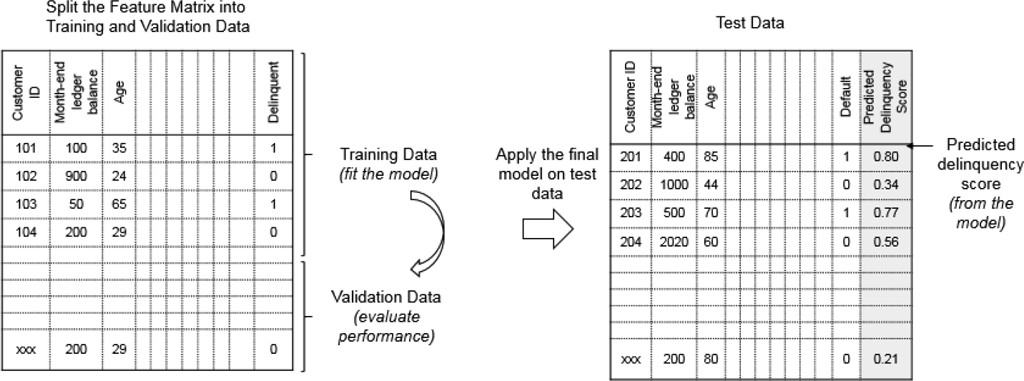
\includegraphics[width=\textwidth,height=0.7\textheight,keepaspectratio]{../../Figures/Buoi_02B/Figure 6.7 The modeling process.jpeg}
            \caption{Quy trình Mô hình hóa}
        \end{figure}
    \end{columns}
\end{frame}

% SLIDE 40
\begin{frame}{4.9 Đánh giá Mô hình (Model Evaluation)}
    \begin{itemize}
        \item Phân tích lỗi (Error Analysis) là bắt buộc.
        \item \textbf{Bài toán Phân loại:} Sử dụng \textbf{Ma trận nhầm lẫn (Confusion Matrix)} so sánh dự đoán Đúng/Sai với mục tiêu thực.
        \begin{itemize}
            \item Các chỉ số: \textit{Accuracy} (Độ chính xác chung), \textit{Precision} (Độ chính xác dương), \textit{Recall} (Độ bao phủ/Độ nhạy).
        \end{itemize}
        \item \textbf{Bài toán Hồi quy:} Tính độ lệch giữa dự báo số và thực tế.
        \begin{itemize}
            \item Các chỉ số: RMSE (Root Mean Squared Error), MAE (Mean Absolute Error).
        \end{itemize}
    \end{itemize}
\end{frame}

% SLIDE 41
\begin{frame}{4.10 Phân tích Lỗi: Độ lệch (Bias) \& Phương sai (Variance)}
    \begin{columns}
        \column{0.55\textwidth}
        \begin{itemize}
            \item \textbf{Lỗi không thể khử (Irreducible Error):} Sai số nhiễu không thể tránh (Bayes error).
            \item \textbf{Độ lệch (Bias):} Lỗi do giả định mô hình sai (Underfitting). Mô hình luôn "chệch" một khoảng cách lớn so với mục tiêu thực sự ở tâm (Tâm bia).
            \item \textbf{Phương sai (Variance):} Lỗi do mô hình ghi nhớ cả dữ liệu nhiễu (Overfitting). Sự phân tán rộng của các điểm dự đoán.
        \end{itemize}
        
        \column{0.45\textwidth}
        \begin{figure}
            \centering
            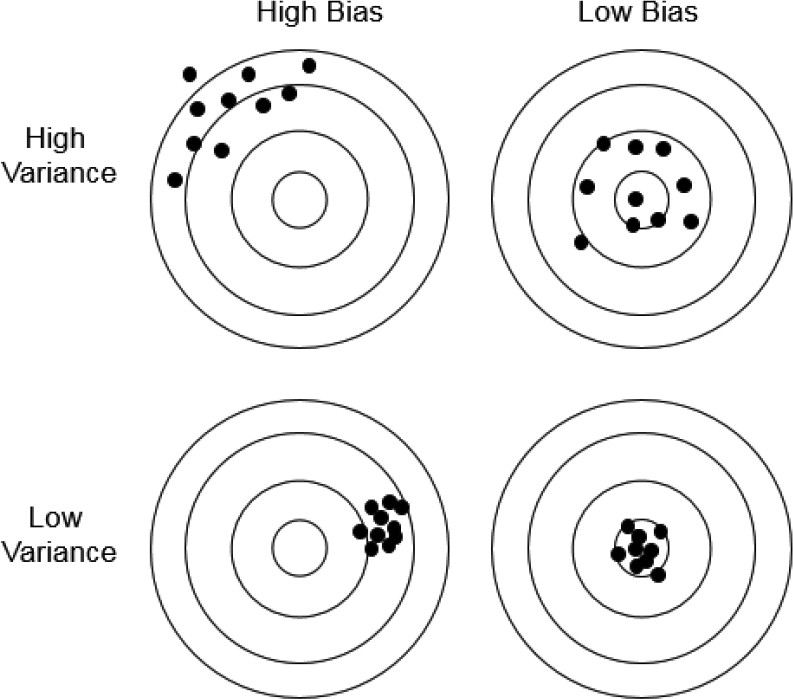
\includegraphics[width=\textwidth,height=0.7\textheight,keepaspectratio]{../../Figures/Buoi_02B/Figure 6.8 Understanding bias and variance.jpeg}
            \caption{Mô phỏng Bias \& Variance}
        \end{figure}
    \end{columns}
\end{frame}

% SLIDE 42
\begin{frame}{4.11 Ngăn xếp Công nghệ Big Data (Technology Stack)}
    \begin{columns}
        \column{0.5\textwidth}
        \begin{itemize}
            \item \textbf{Công cụ Đưa Dữ liệu vào (Ingestion):}
            \begin{itemize}
                \item \textbf{Apache Kafka:} Dòng dữ liệu thời gian thực (Streaming), ví dụ Giao dịch chứng khoán (HFT).
                \item \textbf{Sqoop / Flume:} Chuyển lô dữ liệu từ CSDL truyền thống (RDBMS).
            \end{itemize}
            \item \textbf{Công cụ Xử lý Dữ liệu:} Spark, Pandas, SQL.
        \end{itemize}
        
        \column{0.5\textwidth}
        \begin{figure}
            \centering
            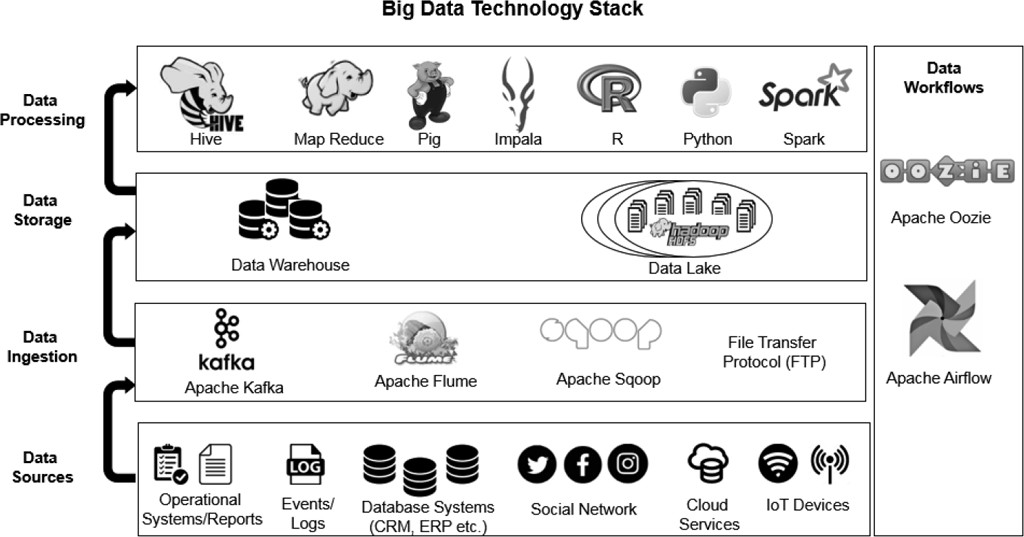
\includegraphics[width=\textwidth,height=0.65\textheight,keepaspectratio]{../../Figures/Buoi_02B/Figure 6.11 The big data technology stack.jpeg}
            \caption{Công nghệ Dữ liệu lớn}
        \end{figure}
    \end{columns}
\end{frame}

% SLIDE 43
\begin{frame}{4.12 Lưu trữ Dữ liệu: Data Warehouse vs. Data Lake}
    \begin{itemize}
        \item \textbf{Kho Dữ liệu (Data Warehouse):}
        \begin{itemize}
            \item Kho lưu trữ tập trung, dữ liệu có cấu trúc chặt chẽ, phải tuân theo lược đồ bảng định trước (Schema).
            \item Dữ liệu kém chất lượng bị loại bỏ. Tối ưu cho truy vấn, báo cáo tài chính ổn định.
        \end{itemize}
        \item \textbf{Hồ Dữ liệu (Data Lake):}
        \begin{itemize}
            \item Triết lý: \textbf{"Lưu trữ trước, xử lý sau"}.
            \item Giữ dữ liệu ở định dạng Thô (Raw) kể cả ảnh, text. 
            \item Tối ưu về tính linh hoạt và tiết kiệm chi phí, sử dụng HDFS (Hệ thống tệp phân tán Hadoop). Rất phù hợp cho AI/ML nghiên cứu.
        \end{itemize}
    \end{itemize}
\end{frame}

% SLIDE 44
\begin{frame}{4.13 Thách thức Quản trị trong Dự án Dữ liệu (P1)}
    \begin{itemize}
        \item Khoa học Dữ liệu cần thiết phải có chiến lược quản trị rủi ro rõ ràng.
        \item \textbf{Quyền riêng tư (Privacy) \& Bảo mật (Security):}
        \begin{itemize}
            \item Quản lý quyền truy cập dữ liệu nhạy cảm theo cấp bậc (Ví dụ: Ai được xem lương, lịch sử y tế?).
            \item Tuân thủ quy định bảo vệ dữ liệu (GDPR Châu Âu, Luật An ninh Mạng VN). Kỹ thuật: Ẩn danh hóa (Anonymization).
        \end{itemize}
        \item \textbf{Đạo đức AI (Ethics):}
        \begin{itemize}
            \item Đảm bảo thuật toán không bị thiên vị (Bias) và phân biệt đối xử (Ví dụ: Chấm điểm tín dụng không dựa trên giới tính, chủng tộc).
        \end{itemize}
    \end{itemize}
\end{frame}

% SLIDE 45
\begin{frame}{4.14 Thách thức Quản trị trong Dự án Dữ liệu (P2)}
    \begin{itemize}
        \item \textbf{Thiếu sự tài trợ (Lack of sponsorships):} 
        \begin{itemize}
            \item Chi phí ban đầu xây dựng kho dữ liệu và tuyển dụng đội ngũ Data Scientist rất tốn kém (Setup cost).
        \end{itemize}
        \item \textbf{Khó khăn khi Triển khai (Deployment):} 
        \begin{itemize}
            \item Rất nhiều mô hình AI thành công trên môi trường thử nghiệm nhưng "chết yểu" khi phải tích hợp (Scale) với các hệ thống kế toán cũ (Legacy Systems).
        \end{itemize}
        \item \textbf{Quản trị Kỳ vọng (Expectation Management):} 
        \begin{itemize}
            \item AI không phải là "Phép thuật". Nó chỉ là công cụ giảm thiểu sự kém hiệu quả và cần thời gian dài để cải thiện độ chính xác.
        \end{itemize}
    \end{itemize}
\end{frame}

% SLIDE 46
\begin{frame}{4.15 Bài tập Ôn tập Tình huống Buổi 2}
    \begin{itemize}
        \item \textbf{Thảo luận Tình huống Ứng dụng Thực tế:}
        \begin{enumerate}
            \item Một ngân hàng nhận thấy hệ thống AI phê duyệt khoản vay từ chối 90\% hồ sơ từ nữ giới trẻ tuổi. Vấn đề này thuộc về Khía cạnh Đạo đức (Ethics) hay Chất lượng Dữ liệu (Veracity), và nhóm Quản trị cần làm gì để điều chỉnh?
            \item Doanh nghiệp của bạn chuẩn bị chuyển đổi số để lưu trữ toàn bộ hóa đơn chứng từ file PDF/Ảnh cùng số liệu kế toán SQL. Giám đốc yêu cầu bạn tư vấn nên chọn xây dựng \textbf{Data Warehouse} (Kho dữ liệu) hay \textbf{Data Lake} (Hồ dữ liệu)? Bạn sẽ tư vấn gì?
        \end{enumerate}
    \end{itemize}
\end{frame}

% SLIDE 47
\begin{frame}{4.16 Tổng kết Buổi 2}
    \begin{itemize}
        \item \textbf{Các điểm Ghi nhớ Cốt lõi:}
        \begin{enumerate}
            \item Tiền mã hóa \& Blockchain (Hợp đồng thông minh) đang tạo ra sổ cái bất biến và minh bạch.
            \item Metaverse và DeFi tạo ra một vũ trụ tài chính mới với AI \& NFT đóng vai trò trung tâm.
            \item Big Data là 4 chữ V (Volume, Velocity, Variety, Veracity). Khoa học Dữ liệu dùng AI/ML như 1 bộ công cụ.
            \item Data Scientist cần kết hợp Toán, Lập trình \& Chuyên môn nghiệp vụ.
            \item Vòng đời dự án bắt đầu từ Định nghĩa vấn đề $\rightarrow$ Chuẩn bị Dữ liệu $\rightarrow$ Lựa chọn Mô hình $\rightarrow$ Đánh giá lỗi (Bias vs. Variance).
        \end{enumerate}
    \end{itemize}
\end{frame}

% SLIDE 48
\begin{frame}{4.17 Chuẩn bị \& Lời dặn dò Buổi 3}
    \begin{itemize}
        \item \textbf{Chuẩn bị Bài học Buổi 3:}
        \begin{itemize}
            \item Đọc trước tài liệu PDF trong thư mục \texttt{textbook} cho Buổi 3: \textbf{"AI and Machine Learning for Accounting"}.
            \item Khảo sát trước cách làm việc với công cụ trực quan hóa dữ liệu (Tableau hoặc PowerBI).
        \end{itemize}
        \item \textbf{Thử thách về nhà:}
        \begin{itemize}
            \item Hãy tìm một bài báo (Ví dụ: trên Vietnambiz, CafeF) bàn về việc ứng dụng Blockchain trong Truy xuất Nguồn gốc chuỗi cung ứng và chia sẻ vào Group Lớp.
        \end{itemize}
    \end{itemize}
\end{frame}

\end{document}
